\chapter{Figure and Table}

\graphicspath{ {graphics/Chapter4/} }

In a scientific document, it is necessary and essential to insert several figures or table to visualize the results.

\section{Insert Images}
	
	\LaTeX~provides several options to handle images and make them look exactly what you need. In this section, some basic operations are explained, e.g. how to include images, how to shrink or enlarge them and how to reference them within your document.
	
	The following code block shows a basic example to insert a figure into the text (see Figure \ref{fig_1}). The explanations for each line of code are also written in the code block. 
	
	\lstset
	{
		language=[LaTeX]TeX,
		breaklines=true,
		basicstyle=\ttfamily\scriptsize,
		keywordstyle=\color{blue},
		moretexcs={\includegraphics},
		xleftmargin=1cm,
		xrightmargin=1cm,
		aboveskip=0\baselineskip
	}

	\begin{lstlisting}
\begin{figure}[h!]
	% position the figure at the horizontal center
	\centering
	% figure width set to 0.75 times the width of text body
	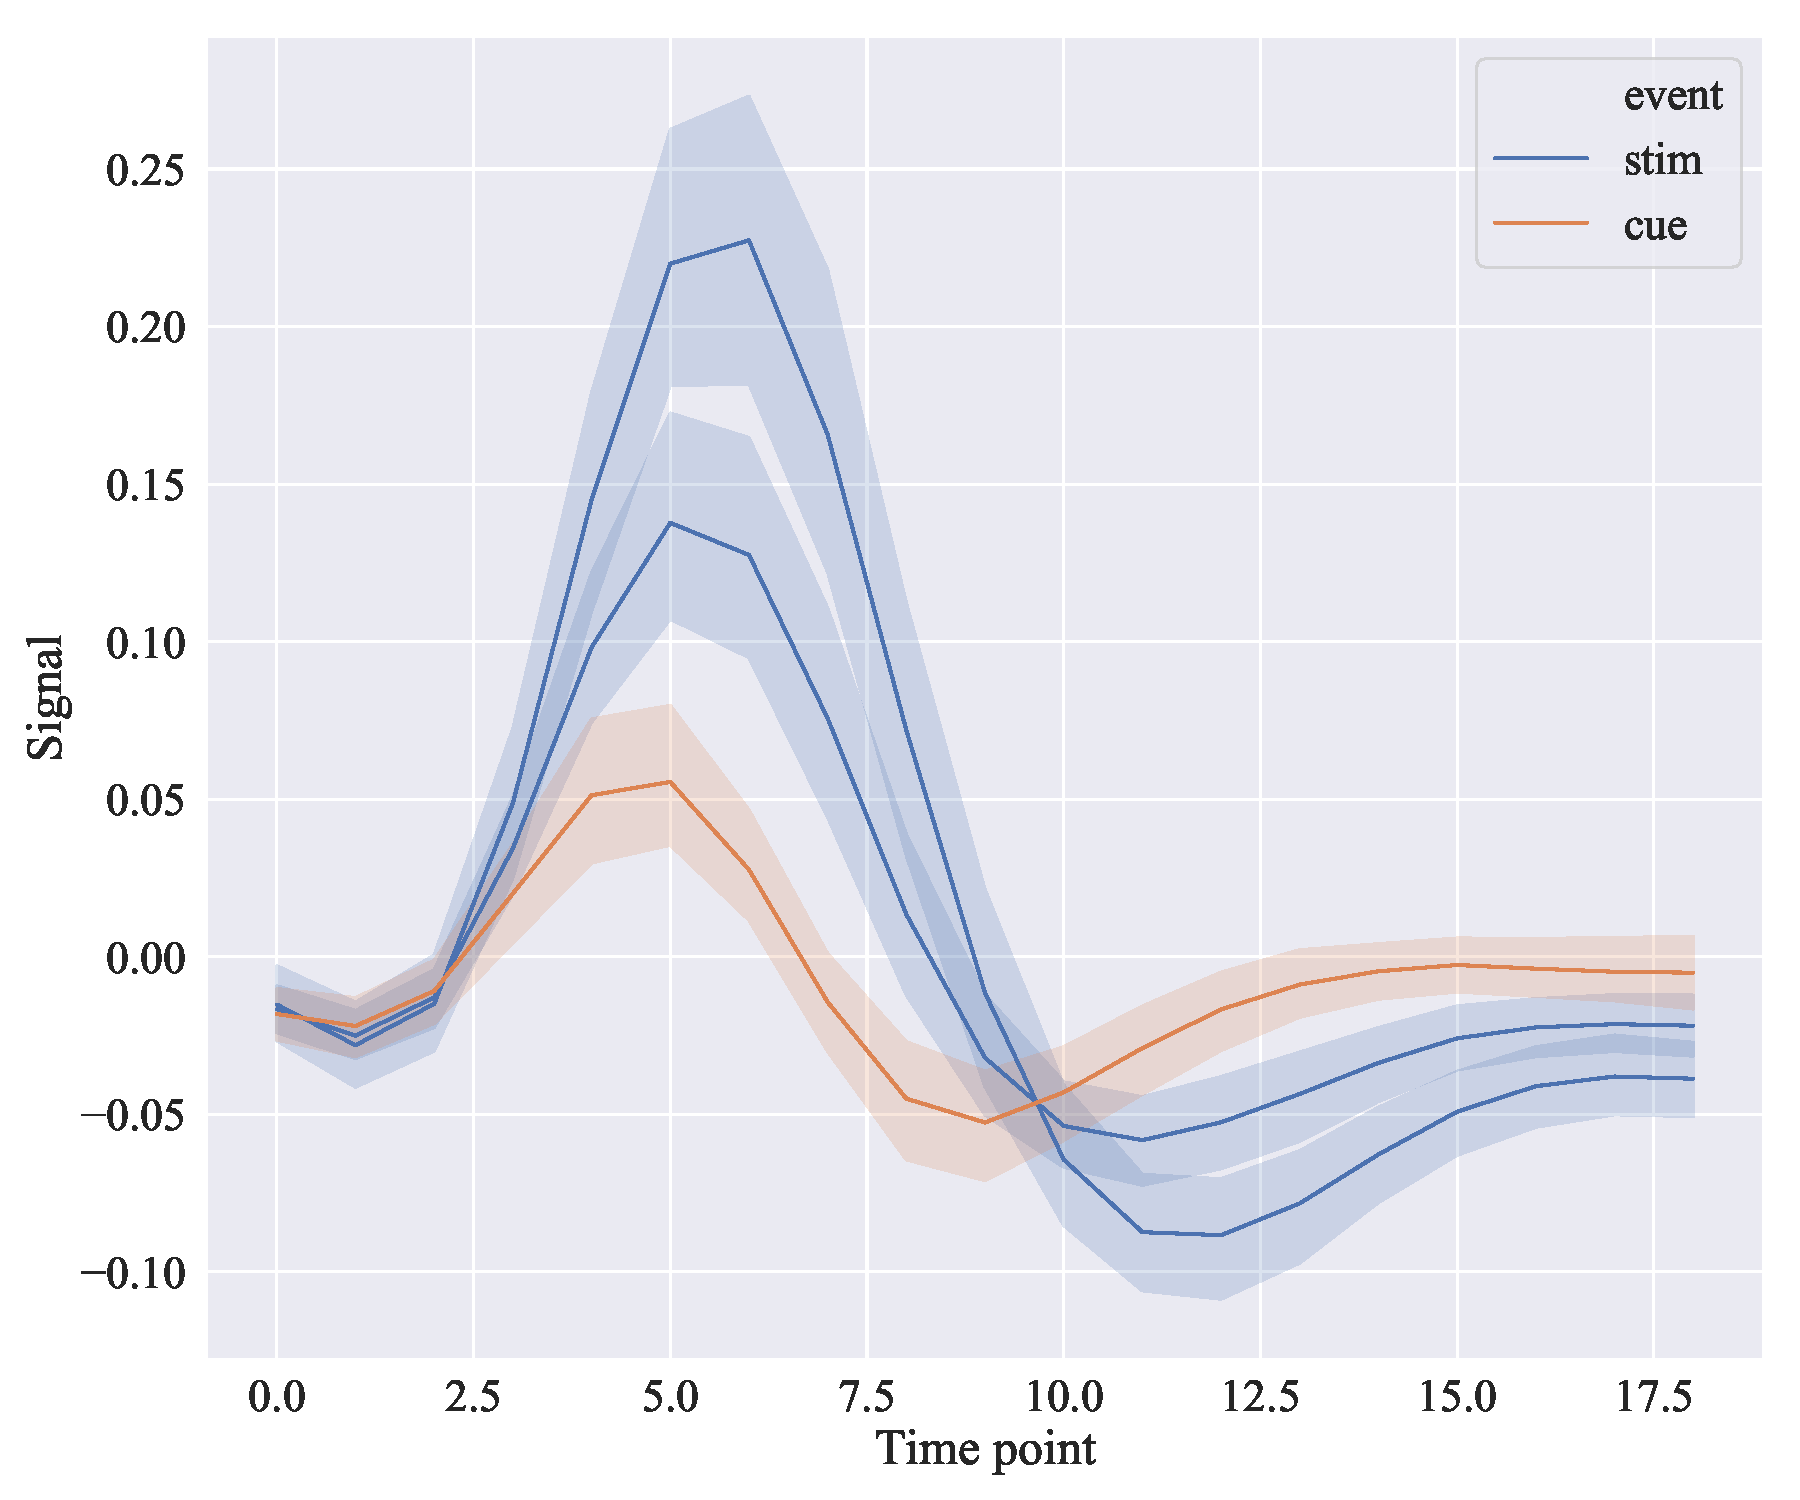
\includegraphics[width=0.75\textwidth]{fig_1.pdf} 
	% set figure caption
	\caption{An exemplary figure} 
	% set label for this figure so it can be refered in the text
	\label{fig_1} 
\end{figure} 
	\end{lstlisting}
	
	\begin{figure}[h!]
		\centering
		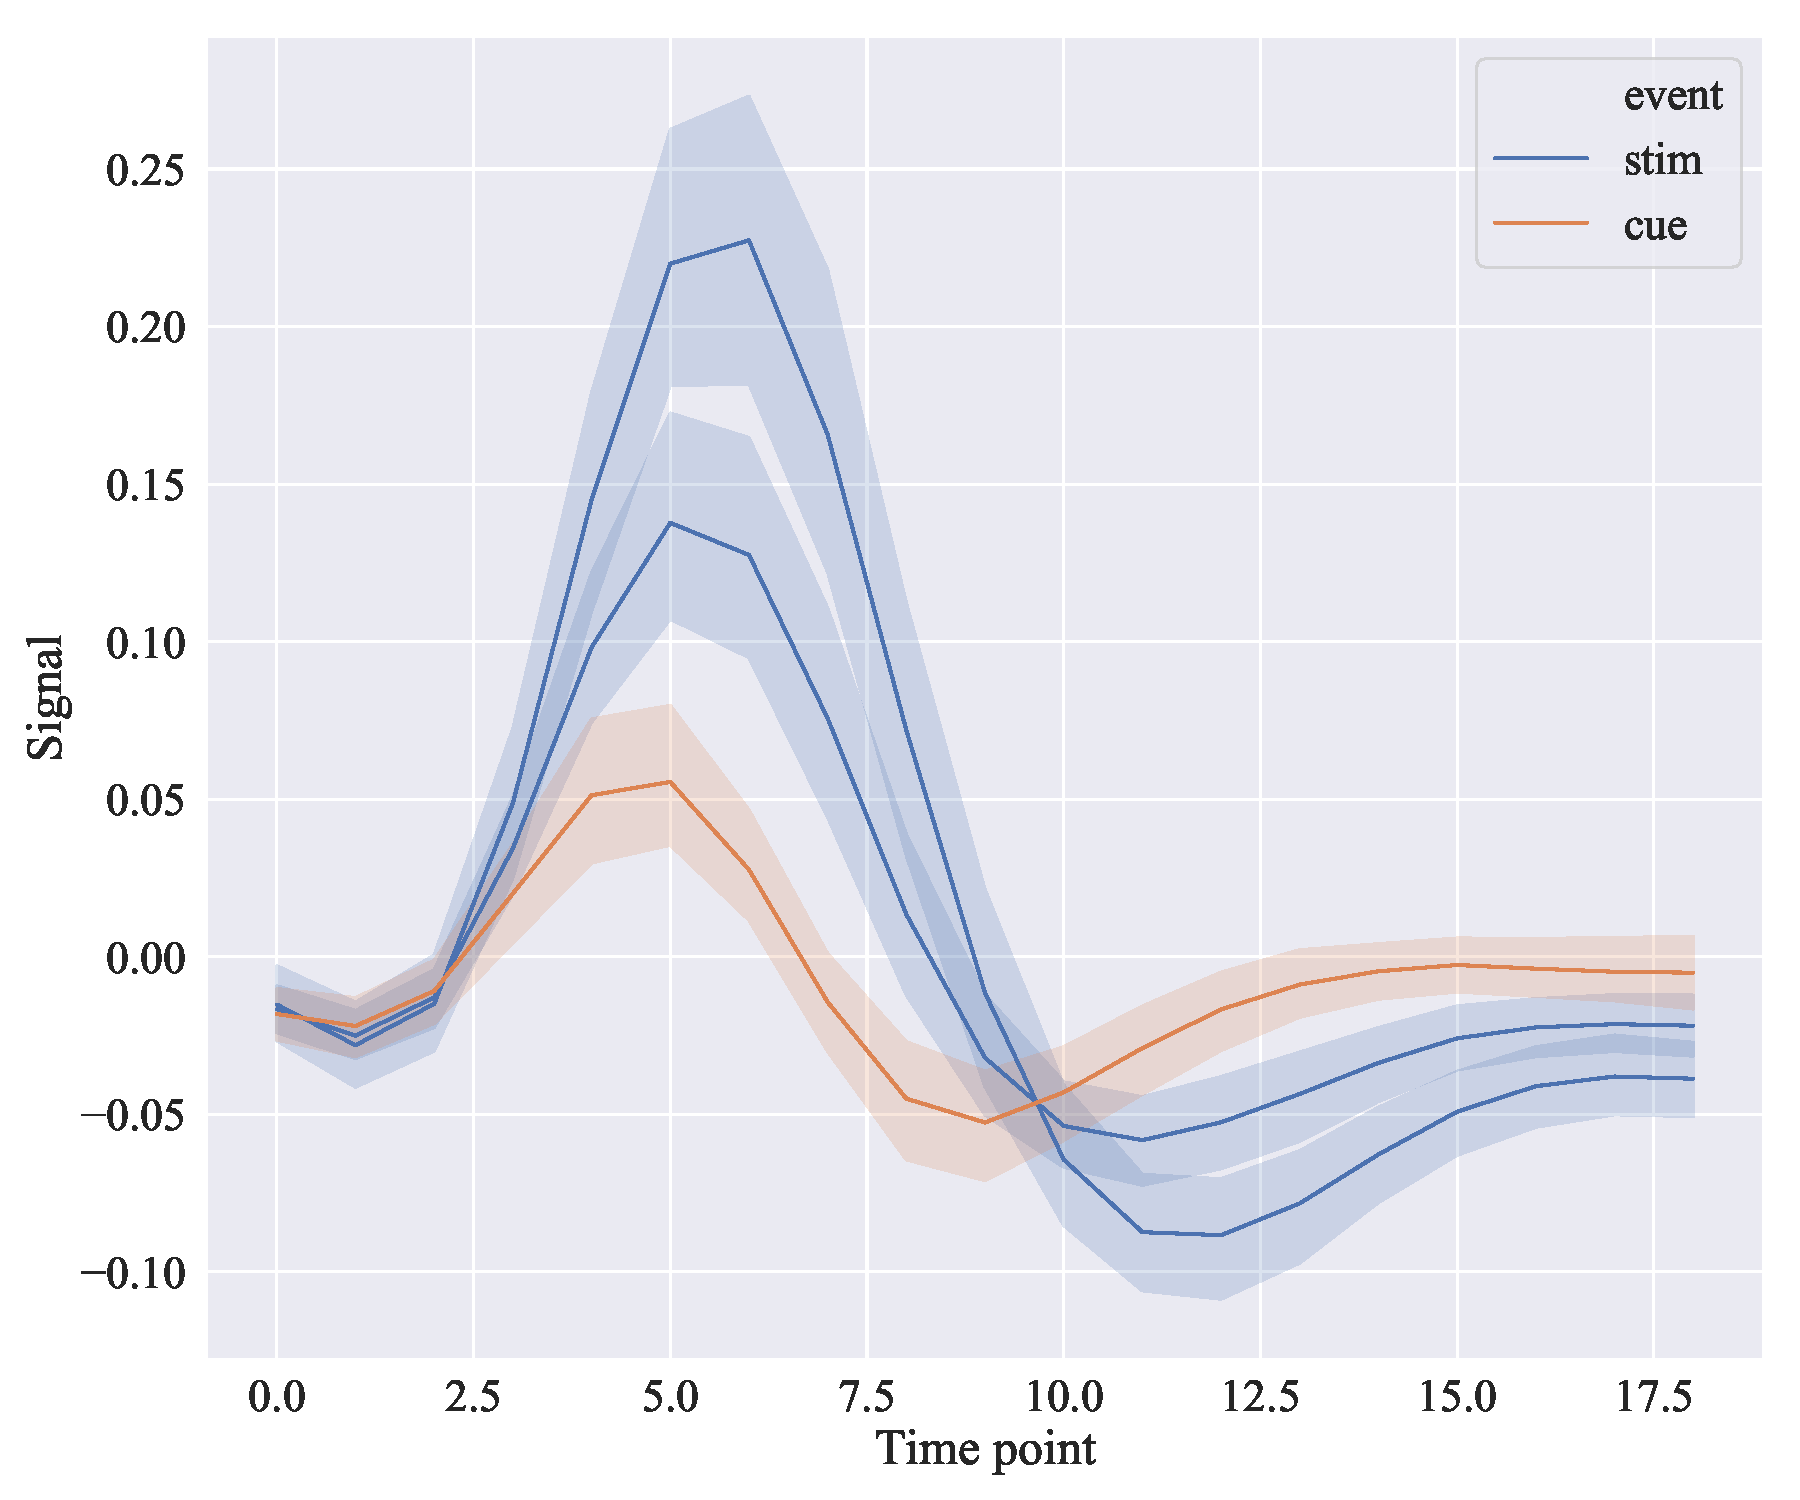
\includegraphics[width=0.75\textwidth]{fig_1.pdf} 
		\caption{An exemplary figure} 
		\label{fig_1} 
	\end{figure} 

	Sometimes one need to insert multiple subplots at once. In \LaTeX~this can be realized by applying the {\color{blue}{\verb|\subfloat|}} environment. In Figure \ref{subfloats}, an example is shown, where four subfigures are included in one figure.
	
	\begin{figure}[h!]
		\centering
		\subfloat{
			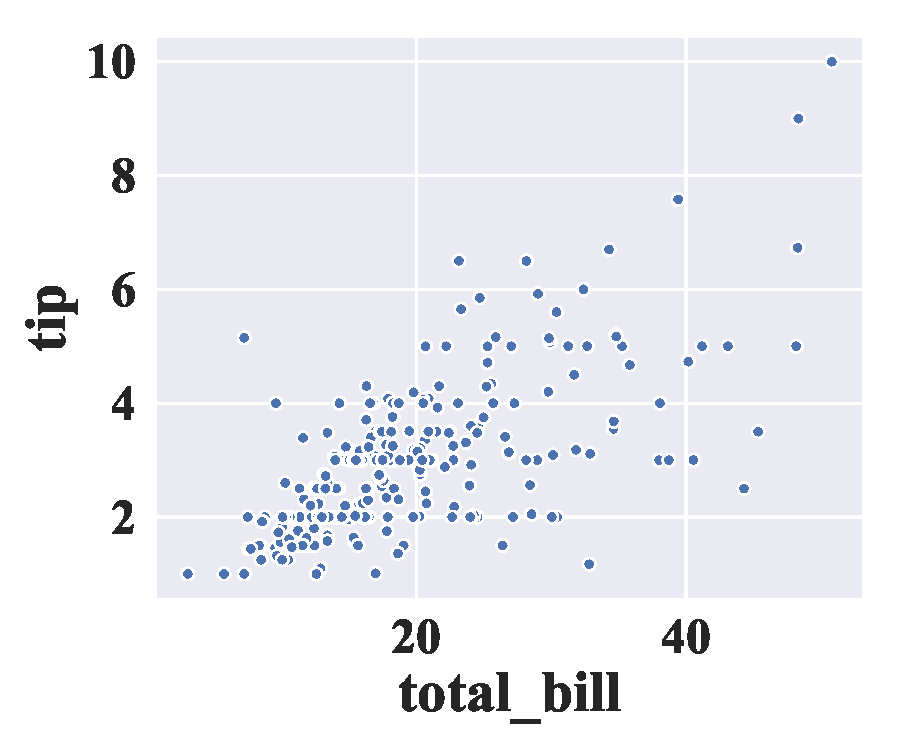
\includegraphics[width=0.375\textwidth]{sub_1.pdf}
			\label{sub_1}
		} \hspace{1cm}
		\subfloat{
			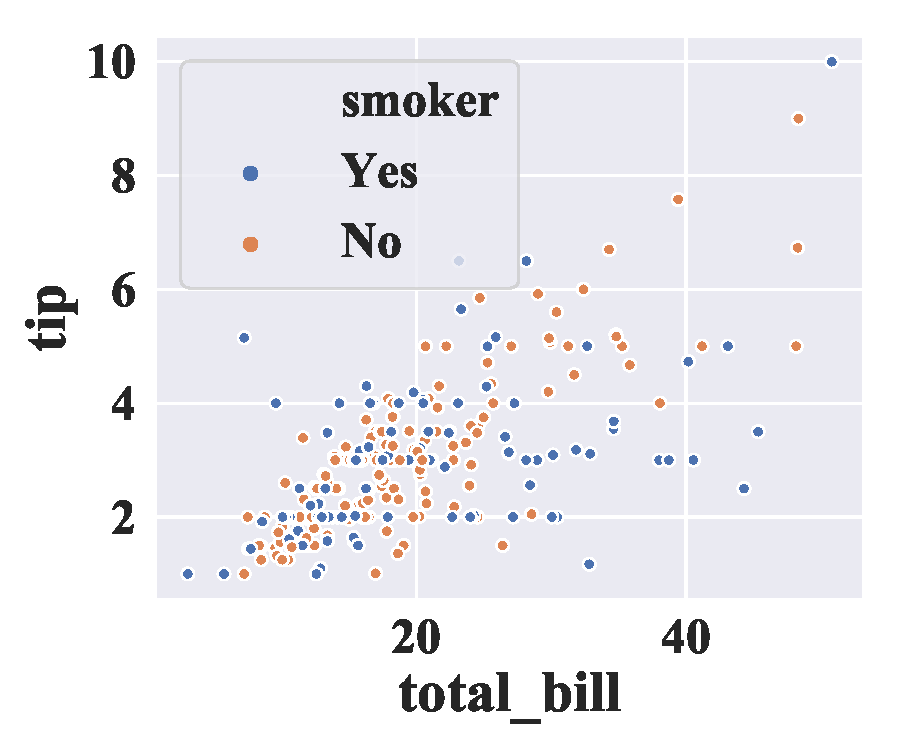
\includegraphics[width=0.375\textwidth]{sub_2.pdf}
		} \\
		\subfloat{
			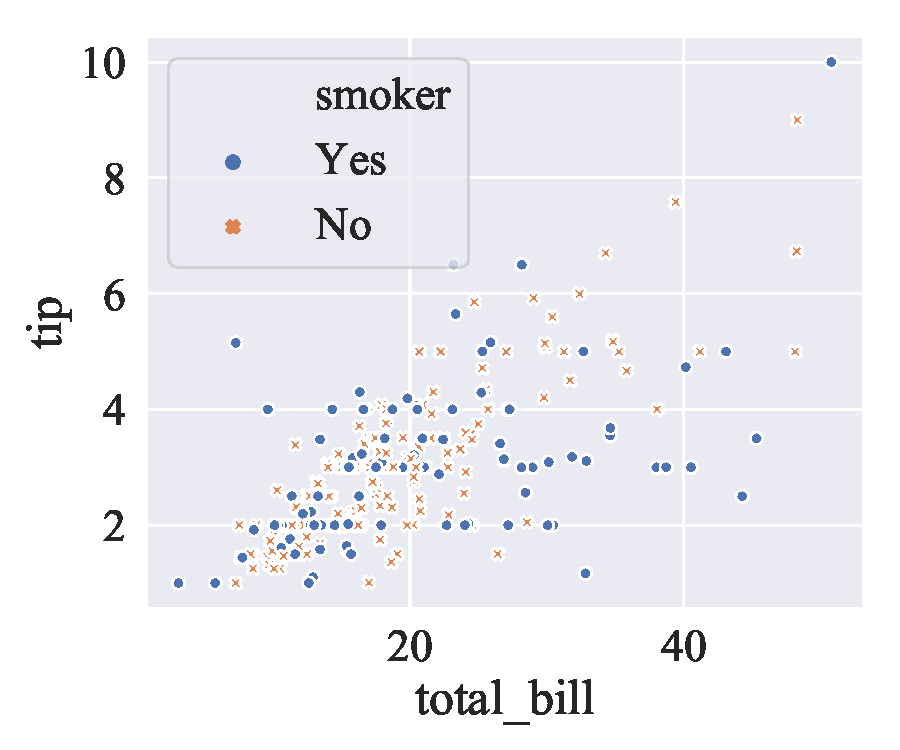
\includegraphics[width=0.375\textwidth]{sub_3.pdf}
			\label{p_diff_tennet}
		}
		\subfloat{
			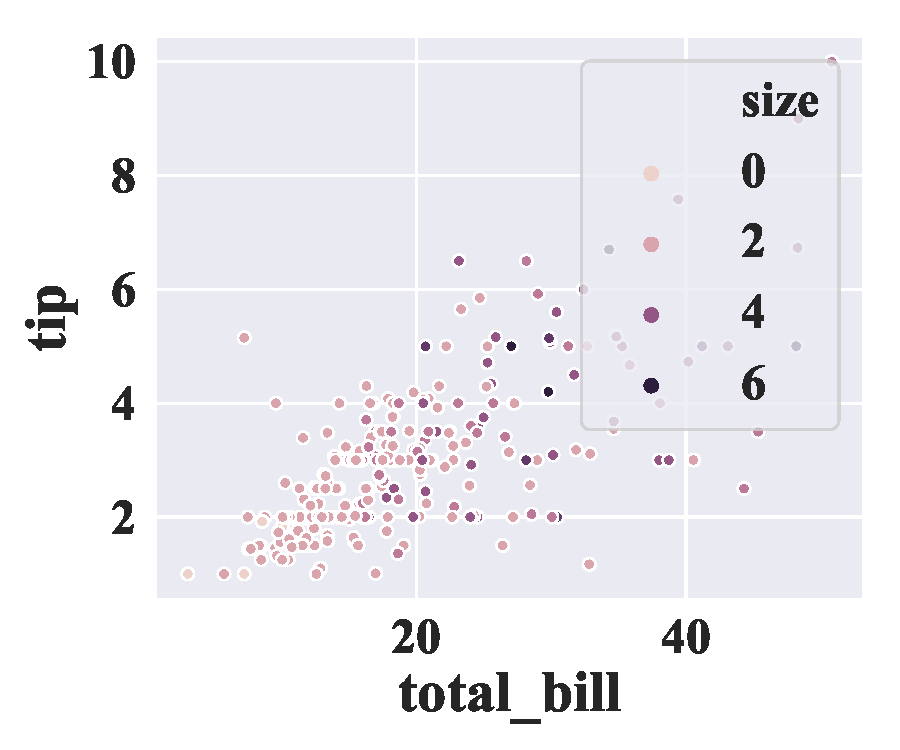
\includegraphics[width=0.375\textwidth]{sub_4.pdf}
			\label{q_diff_tennet}
		}
	\end{figure}

	In this template, all exemplary figures are generated by matplotlib.pyplot library and scaled to wished size in the text. It should be however noticed, that due to the resizing process in \LaTeX, the font size set in original figures may be lost. Therefore, it is important to attempt different font size in your figures generated by software or programming languages. Another option is to utilize the {\color{blue}tikzpicture} package in \LaTeX, which can help to add text description of axes. An example of using {\color{blue}tikzpicture} package to obtain the same figure as Figure \ref{fig_1} is shown in Figure \ref{tikzpic}. You can compare this two figures and refer to the corresponding codes when necessary.
	
	\begin{figure}[h!]
		\centering
		\begin{tikzpicture}
			\node (img)  {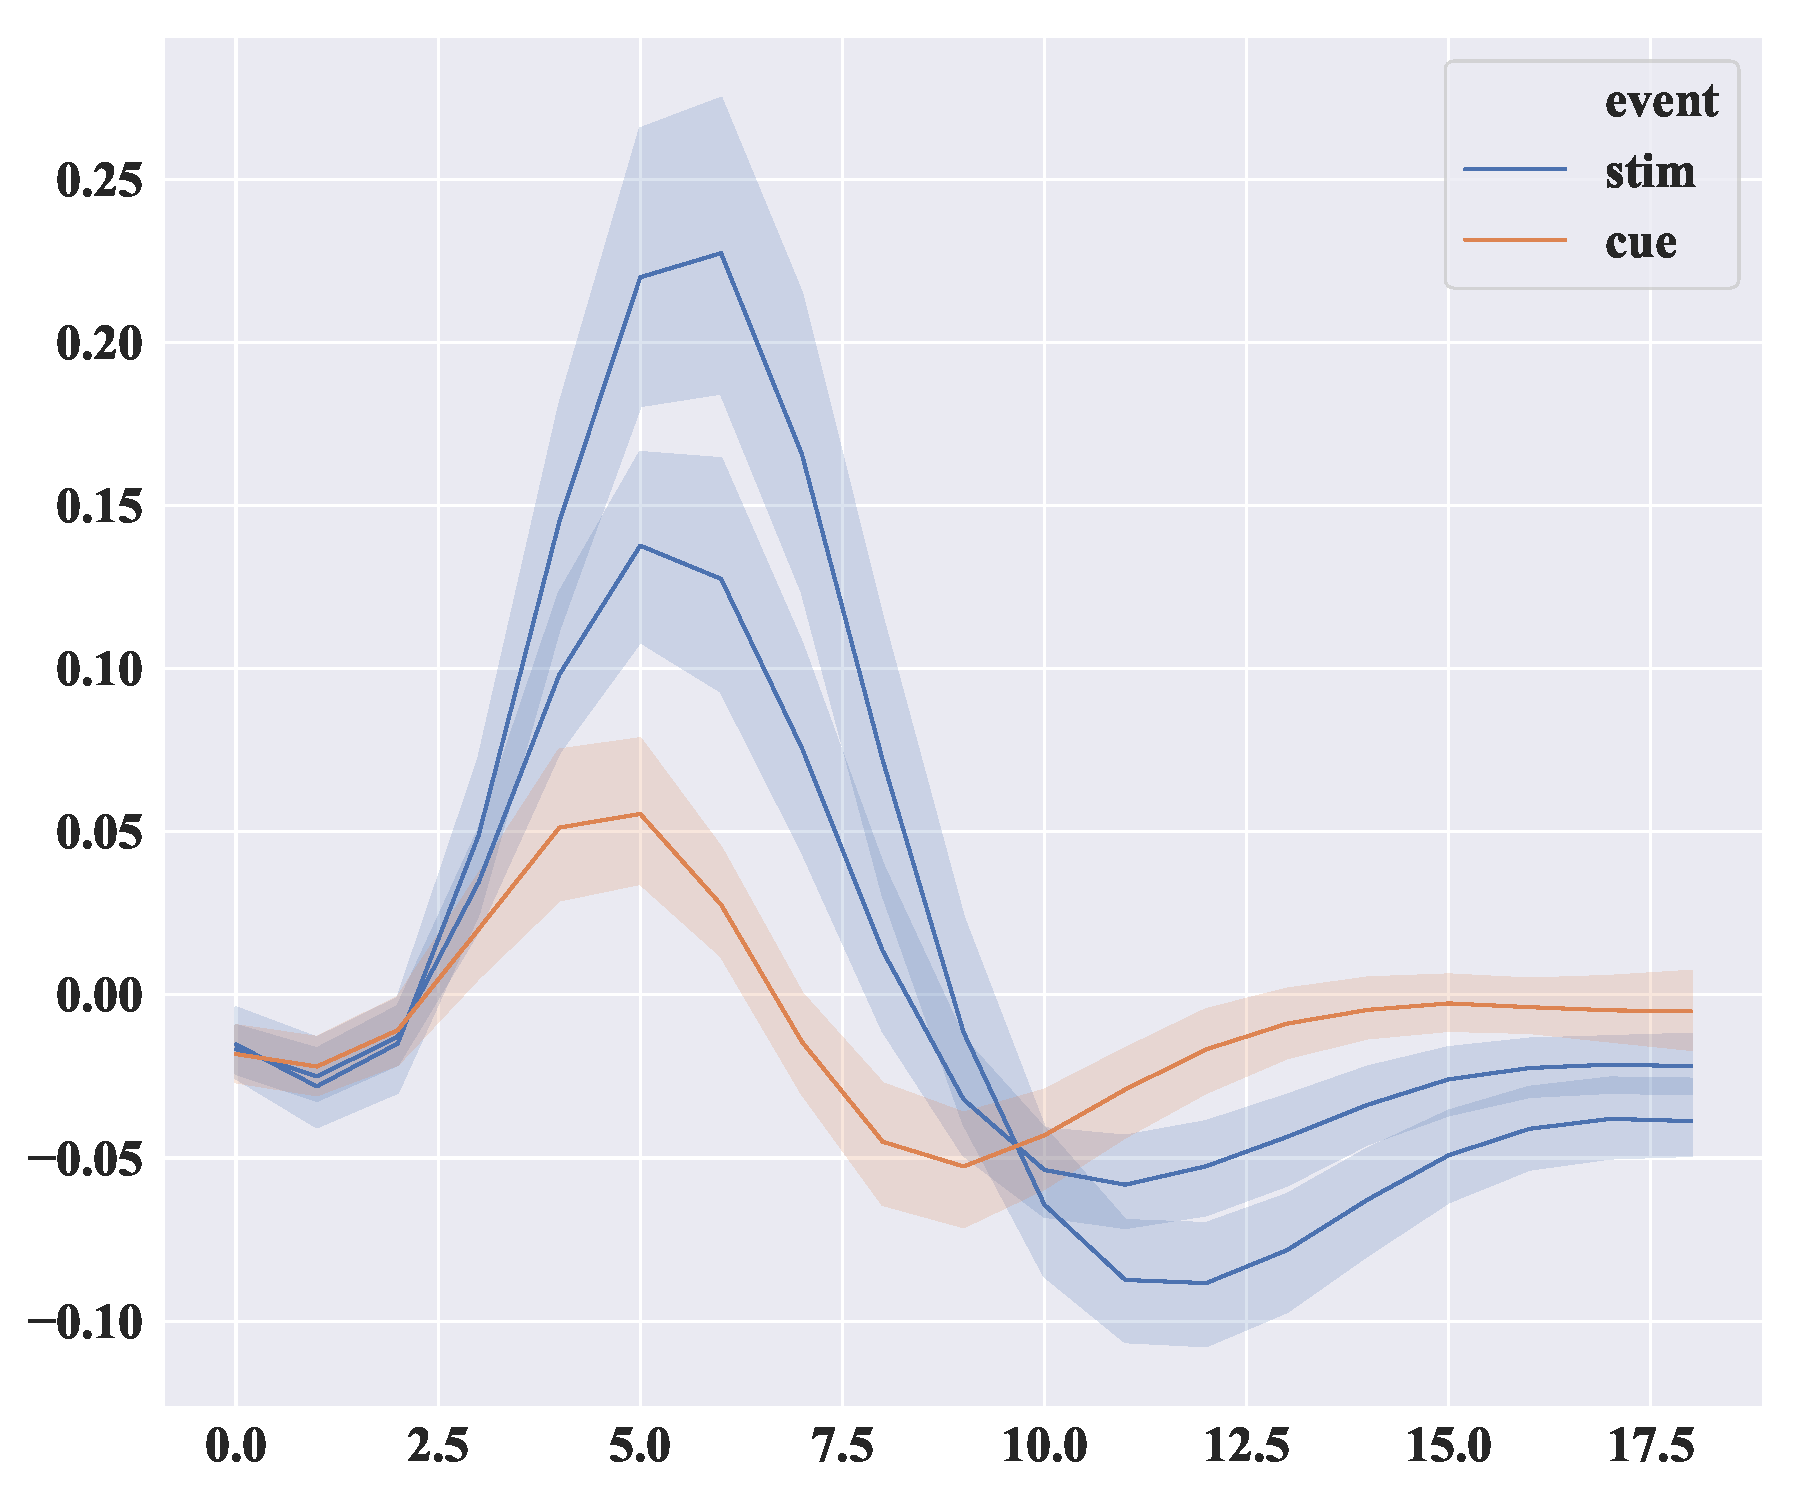
\includegraphics[width=0.75\textwidth]{fig_2.pdf}};
			\node[below=of img, node distance=0cm, yshift=1.2cm,font=\footnotesize] {Time point};
			\node[left=of img, node distance=0cm, rotate=90, anchor=center,yshift=-1cm,font=\footnotesize] {Signal};
		\end{tikzpicture}
		\caption{An example of tikzpicture}
		\label{tikzpic}
	\end{figure}
	
\section{Inserting Tables}

	Table is another common element in scientific documents. \LaTeX provides a large set of tools to customize tables. Some most common types and corresponding commands are shown in this section.
	
	Following code block shows a simple example to create a table. The parameter of command {\color{blue}{\verb|tabular|}} is aimed to set the number of columns, their delimiters and the alignment types. As shown in the exemplary codes, {\color{blue}{\texttt{{| l | c | r |}}}} creates a table with three columns and the ``|" symbols create vertical delimiters in the table. The letters are the definitions of alignment for each column, e.g. ``l" means left alignment, ``c" center and ``r" right. To add horizontal delimiters, just add {\color{blue}{\verb|\hline|}} before or after the entry of a row. 
	
	\begin{lstlisting}
\begin{table}
\centering
	\begin{tabular}{| l | c | r |}
		\hline
		Points per game & Rebounds per game & Assists per game \\ \hline
		7.6  & 1.9 & 1.3 \\ \hline
		15.4 &	3.1	& 2.5 \\ \hline
		19.9 &	5.3 & 3.8 \\ \hline
	\end{tabular}
\end{table}
	\end{lstlisting}
	
	\begin{table}[h!]
		\centering
		\begin{tabular}{| l | c | r |}
			\hline
			Points per game & Rebounds per game & Assists per game \\ \hline
			7.6  & 1.9 & 1.3 \\ \hline
			15.4 & 3.1 & 2.5 \\ \hline
			19.9 & 5.3 & 3.8 \\ \hline
		\end{tabular}
		\caption{An exemplary table}
		\label{table_1}
	\end{table}
	
	Now the parameter {\color{blue}{\texttt{| l  c  r |}}} is used to format columns and some {\color{blue}{\verb|\hline|}} commands are removed, the output table is shown in Table \ref{table_2}.
	
		\begin{table}[h!]
		\centering
		\begin{tabular}{| l  c  r |}
			\hline
			Points per game & Rebounds per game & Assists per game \\ \hline
			7.6  & 1.9 & 1.3 \\ 
			15.4 & 3.1 & 2.5 \\
			19.9 & 5.3 & 3.8 \\ \hline 
		\end{tabular}
		\caption{Another exemplary table}
		\label{table_2}
	\end{table}

	It is sometimes necessary to merge several cells into one to make the table contents more evident. In \LaTeX~this function can be done by using {\verb|\multicolumn{text}{pos}{text}|} or {\verb|\multirow{text}{width}{text}|} commands.

	
	\begin{table}
		\centering
		\rowcolors{5}{purple!20}{yellow!20}
		\begin{tabularx}{0.9\textwidth}{| c | X | X | X | X | X | X |}
			
			Season  & MPG  & PPG  &	RPG & APG &	SPG & BPG \\
			1996–97 & 15.5 & 7.6  & 1.9 & 1.3 &  .7	&  .3 \\
			1997–98	& 26.0 & 15.4 &	3.1	& 2.5 &	 .9	&  .5 \\
			1998–99	& 37.9 & 19.9 &	5.3 & 3.8 &	1.4	& 1.0 \\
			1999–00	& 38.2 & 22.5 &	6.3	& 4.9 &	1.6	&  .9 \\
			2000–01 & 40.9 & 28.5 &	5.9	& 5.0 &	1.7 &  .6 \\
			2001–02 & 38.3 & 25.2 &	5.5	& 5.5 &	1.5	&  .4 \\
			2002–03 & 41.5 & 30.0 &	6.9	& 5.9 &	2.2	&  .8 \\
			2003–04	& 37.6 & 24.0 &	5.5	& 5.1 &	1.7	&  .4 \\
			2004–05	& 40.7 & 27.6 &	5.9	& 6.0 &	1.3 &  .8 \\
			2005–06	& 41.0 & 35.4 &	5.3	& 4.5 &	1.8 &  .4 \\
			2006–07	& 40.8 & 31.6 &	5.7	& 5.4 &	1.4	&  .5 \\
			2007–08	& 38.9 & 28.3 &	6.3	& 5.4 &	1.8	&  .5 \\
			2008–09	& 36.1 & 26.8 &	5.2	& 4.9 &	1.5	&  .5 \\
			2009–10	& 38.8 & 27.0 &	5.4	& 5.0 &	1.5	&  .3 \\
			2010–11	& 33.9 & 25.3 &	5.1	& 4.7 &	1.2	&  .1 \\
			2011–12	& 38.5 & 27.9 &	5.4	& 4.6 &	1.2	&  .3 \\
			2012–13	& 38.6 & 27.3 &	5.6	& 6.0 &	1.4	&  .3 \\
			2013–14	& 29.5 & 13.8 &	4.3	& 6.3 &	1.2	&  .2 \\
			2014–15	& 34.5 & 22.3 &	5.7	& 5.6 &	1.3	&  .2 \\
			2015–16	& 28.2 & 17.6 &	3.7	& 2.8 &	.9	&  .2 \\
			Career	& 36.1 & 25.0 &	5.2	& 4.7 &	1.4	&  .5 \\
		\end{tabularx}
	\end{table}